\appendix
\renewcommand{\thetable}{S\arabic{table}}
\setcounter{table}{0}
\section{补充材料}

\subsection{输入特征与参数候选}

% Word body block 127
基础配置的 19 个字段依次为：修饰/官能团信息、合成方法、表面电荷、细胞类型、细胞组织、发表年份、最终粒径、最终 Zeta 电位、Zeta 绝对值、暴露时间、历史浓度、log(1 + 粒径)、log(1 + 时间)、log(1 + 浓度)、接种细胞数，以及 Zeta、细胞数、修饰信息和表面电荷的四个缺失标志。化学候选为 Se 含量、稳定性时间、Se 3d 结合能和晶体学报告状态，IC50 配置额外考虑历史实测 IC50 。晶体学报告状态使用原晶体学字段是否非空构造，不是测定晶相的替代值。

% Word body block 128
RF 候选（树数、最大深度、叶节点最小样本数）为（250、不限、2）、（250、10、2）和（250、不限、4）；XGBoost 候选（轮次、最大深度、学习率）为（150、2、0.05）、（250、2、0.05）和（250、3、0.05）。固定预算通用与迁移对照使用 500 树预算，RF 的最小叶节点样本数为 2，XGBoost 的最大深度为 3、学习率为 0.05，其余固定参数与方法部分一致。

\subsection{完整配对增量结果}

% Word body block 130
表 S1 同时列出样本等权差值与文献组等权差值，区间对应后者。基础嵌套分析中归档的逐样本 bootstrap 指标区间属于另一不确定性口径，本稿不将它们写成文献组区间，也不将通用基准中的组等权区间直接附到样本等权性能数值上。

% Word body block 132: 表格逐单元格转写。
\begin{table}[H]
\centering
\caption{各配置相对对应基线的配对 MAE 差值，单位为存活率百分点。负值表示误差下降，区间来自 24 个文献组等权差值的 5000 次 bootstrap。}
\label{tab:paired_comparisons}
\small
\begin{tabularx}{\linewidth}{lXrrr}
\toprule
模型 & 对照 & \ensuremath{\Delta}MAE 样本等权 & \ensuremath{\Delta}MAE 文献组等权 & 文献组等权 95\% 区间 \\
\midrule
RF & 化学增强 & +0.180 & +0.183 & [0.054, 0.333] \\
XGBoost & 化学增强 & +0.030 & \ensuremath{\mathord{-}}0.049 & [\ensuremath{\mathord{-}}0.822, 0.668] \\
RF & IC50 辅助 & \ensuremath{\mathord{-}}0.142 & \ensuremath{\mathord{-}}0.326 & [\ensuremath{\mathord{-}}3.285, 2.542] \\
XGBoost & IC50 辅助 & \ensuremath{\mathord{-}}1.145 & \ensuremath{\mathord{-}}0.835 & [\ensuremath{\mathord{-}}3.296, 1.531] \\
RF & 加入剂量—时间交互 & +0.392 & +0.415 & [\ensuremath{\mathord{-}}0.072, 1.102] \\
XGBoost & 加入剂量—时间交互 & +0.605 & +0.388 & [\ensuremath{\mathord{-}}0.199, 1.016] \\
RF & General\ensuremath{\rightarrow}SeNP 迁移 & +0.577 & \ensuremath{\mathord{-}}0.535 & [\ensuremath{\mathord{-}}2.763, 1.414] \\
XGBoost & General\ensuremath{\rightarrow}SeNP 迁移 & \ensuremath{\mathord{-}}0.669 & \ensuremath{\mathord{-}}0.054 & [\ensuremath{\mathord{-}}1.417, 1.317] \\
\bottomrule
\end{tabularx}

\end{table}

\subsection{27 条曲线的表观 IC50}

% Word body block 135
表 S2 覆盖全部九种材料与三个时间点，不删除测试范围内未达到阈值的曲线。所有有限值均为对数浓度相邻点插值，单位沿用待核实的原始浓度尺度，显示两位小数仅用于一致排版，不表示相应的测量精度；> 512 只记录阈值未检出。该表不包含模型预测 IC50 或预测—实测误差。

% Word body block 137: 表格逐单元格转写。
\begin{table}[H]
\centering
\caption{HUVEC 材料—时间曲线的表观 IC50，采用原始浓度尺度。重复次数与汇总方法待核实。}
\label{tab:huvec_ic50}
\small
\begin{tabular}{lrrr}
\toprule
材料 & 24 h & 48 h & 72 h \\
\midrule
CS-SeNPs & $>512$ & 20.90 & 11.94 \\
Glucose-SeNPs & $>512$ & 185.33 & 24.89 \\
LET-SeNPs & 281.86 & 39.55 & 11.63 \\
PAH-SeNPs & 30.22 & 26.84 & 25.00 \\
PEG-SeNPs & $>512$ & 28.48 & 27.41 \\
PEI-SeNPs & $>512$ & 448.56 & 323.37 \\
PVP-SeNPs & $>512$ & 60.65 & 30.59 \\
Sucrose-SeNPs & $>512$ & $>512$ & 323.74 \\
TW80-SeNPs & $>512$ & 15.68 & 14.30 \\
\bottomrule
\end{tabular}

\end{table}

\subsection{新增实验源数据的使用规则}

% Word body block 140
新增实验原始报告字段为材料名称、粒径（nm）、Zeta 电位（mV）、细胞类型、浓度报告值、时间（h）和存活率（\%）351 条记录完整覆盖所有材料—时间—浓度组合，保留零浓度对照、60个大于 100\% 的存活率报告值与局部非单调响应，不做删点、额外归一化或浓度换算。材料比较表、时间汇总表、表观 IC50 的相邻括区与描述符相关系数均由归档 CSV 重新生成，原始工作簿与 CSV 的一致性以归档哈希及逐值核验为依据。

% Word body block 141
既有随机划分复现用于追溯历史报告，包含不同预处理和全量拟合指标，不进入本稿的主模型排名。原计划的修饰类别—分子量信息层级、可靠配方分组、完整材料表征与模型前瞻盲测，按当前归档可支持的范围记录，不将未生成的指标或未提供的数据补写为已完成结果。

\FloatBarrier
\section*{内部核验附录：暂不纳入正式正文的图件}

% Word body block 143
以下两张图随本轮材料一并保存，供作者核查，不应作为已验证的正式论文结果图直接投稿。IAE 热图的积分定义和完整计算脚本尚未核实。IC50 配对散点图中的预测 IC50 数值与逐条件预测曲线不一致：27 条预测曲线的最低预测存活率均高于 50\%，因此不能从当前预测曲线直接插值得到图中所示的有限模型 IC50。

% Word body blocks 144–145: 嵌入图保持原始字节。
\begin{figure}[H]
\centering
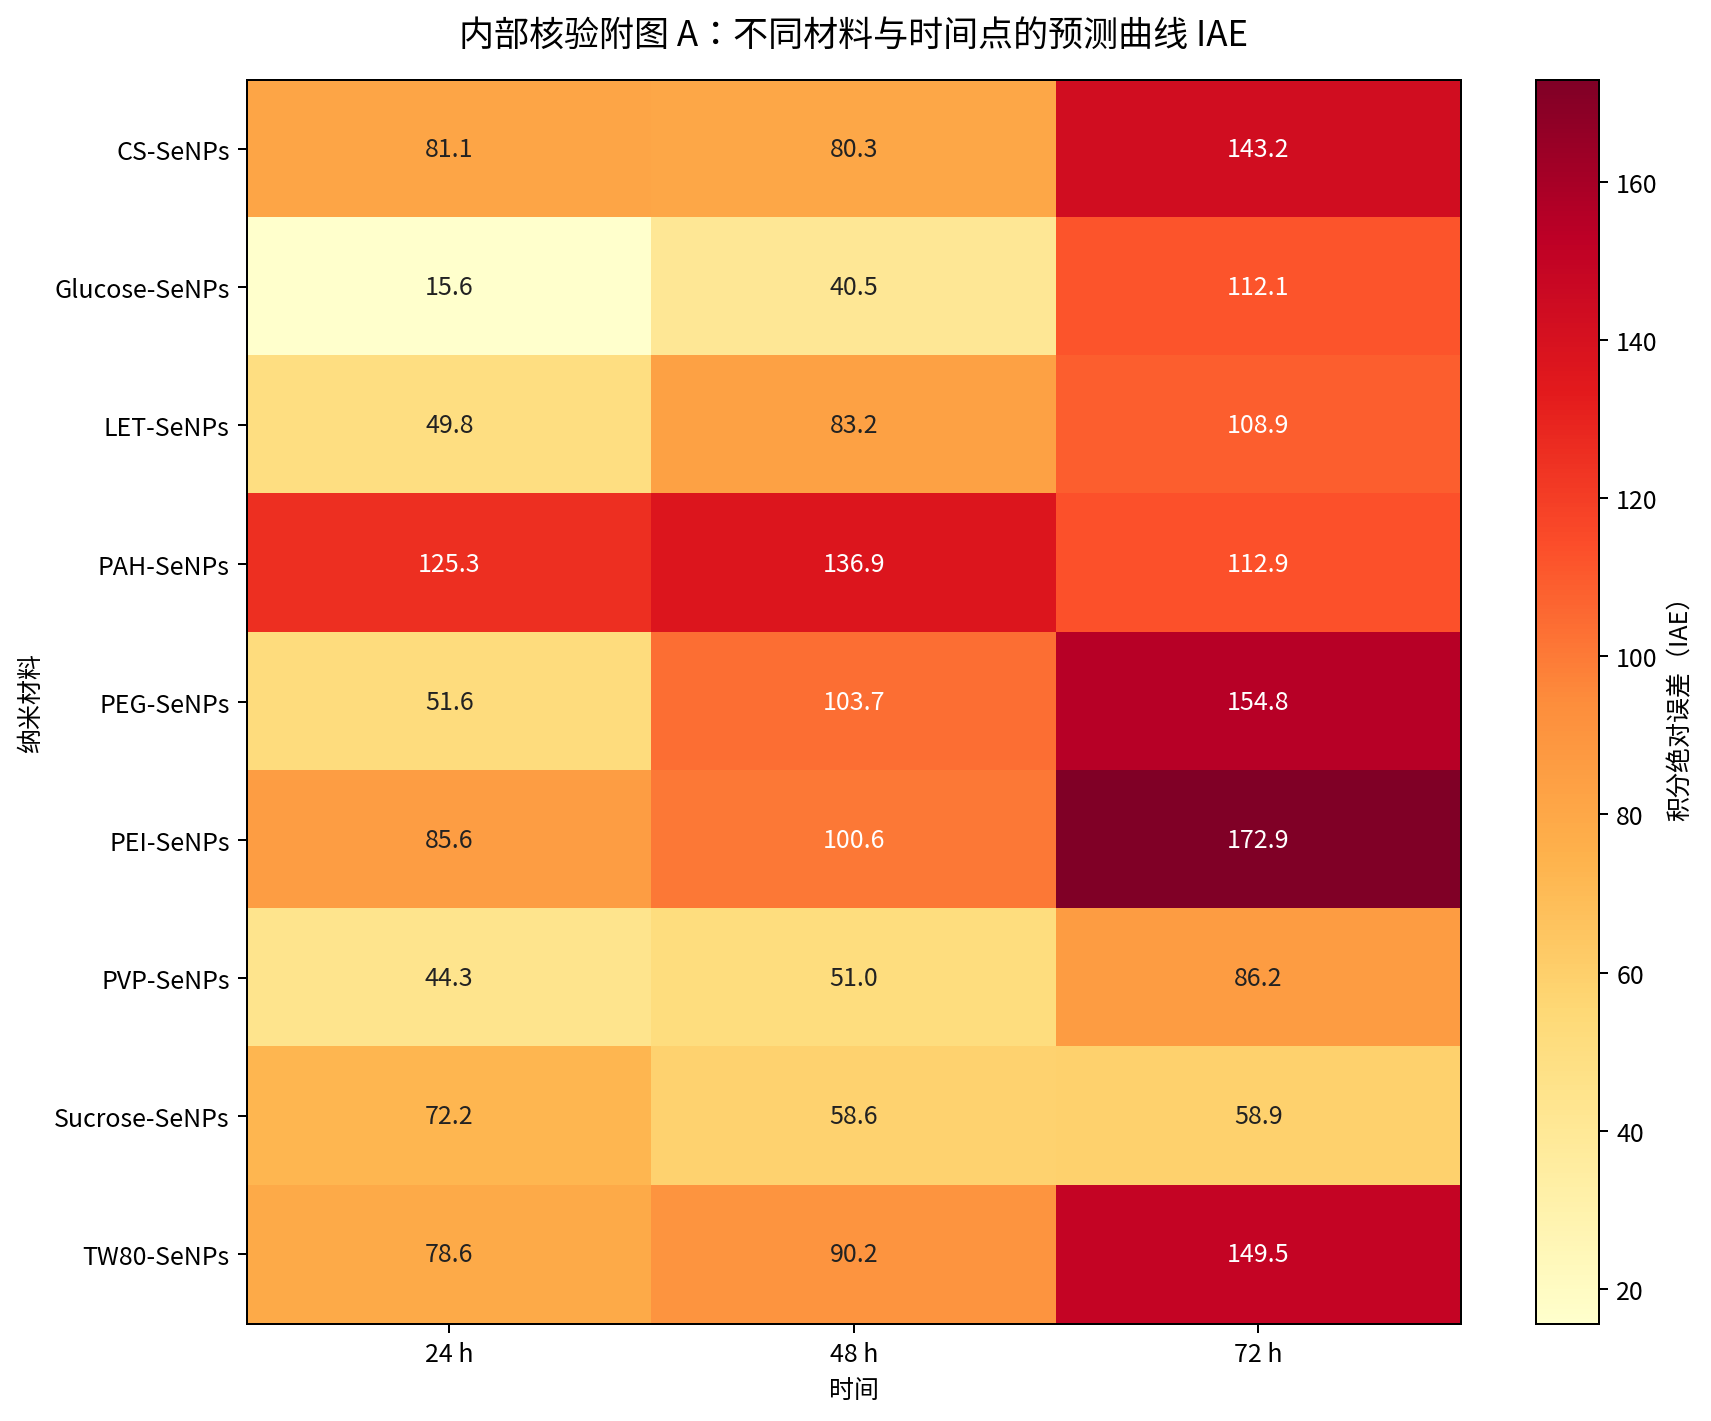
\includegraphics[width=\linewidth,height=0.70\textheight,keepaspectratio]{figures/word-20261021/iae-heatmap.png}
\caption*{内部核验附图 A. 任务 24 的 IAE 热图。暂不纳入正式正文，待核对积分横轴、零浓度处理、积分区间和数值积分方法后再决定。}
\label{fig:huvec_internal_iae}
\end{figure}

% Word body blocks 146–147: 嵌入图保持原始字节。
\begin{figure}[H]
\centering
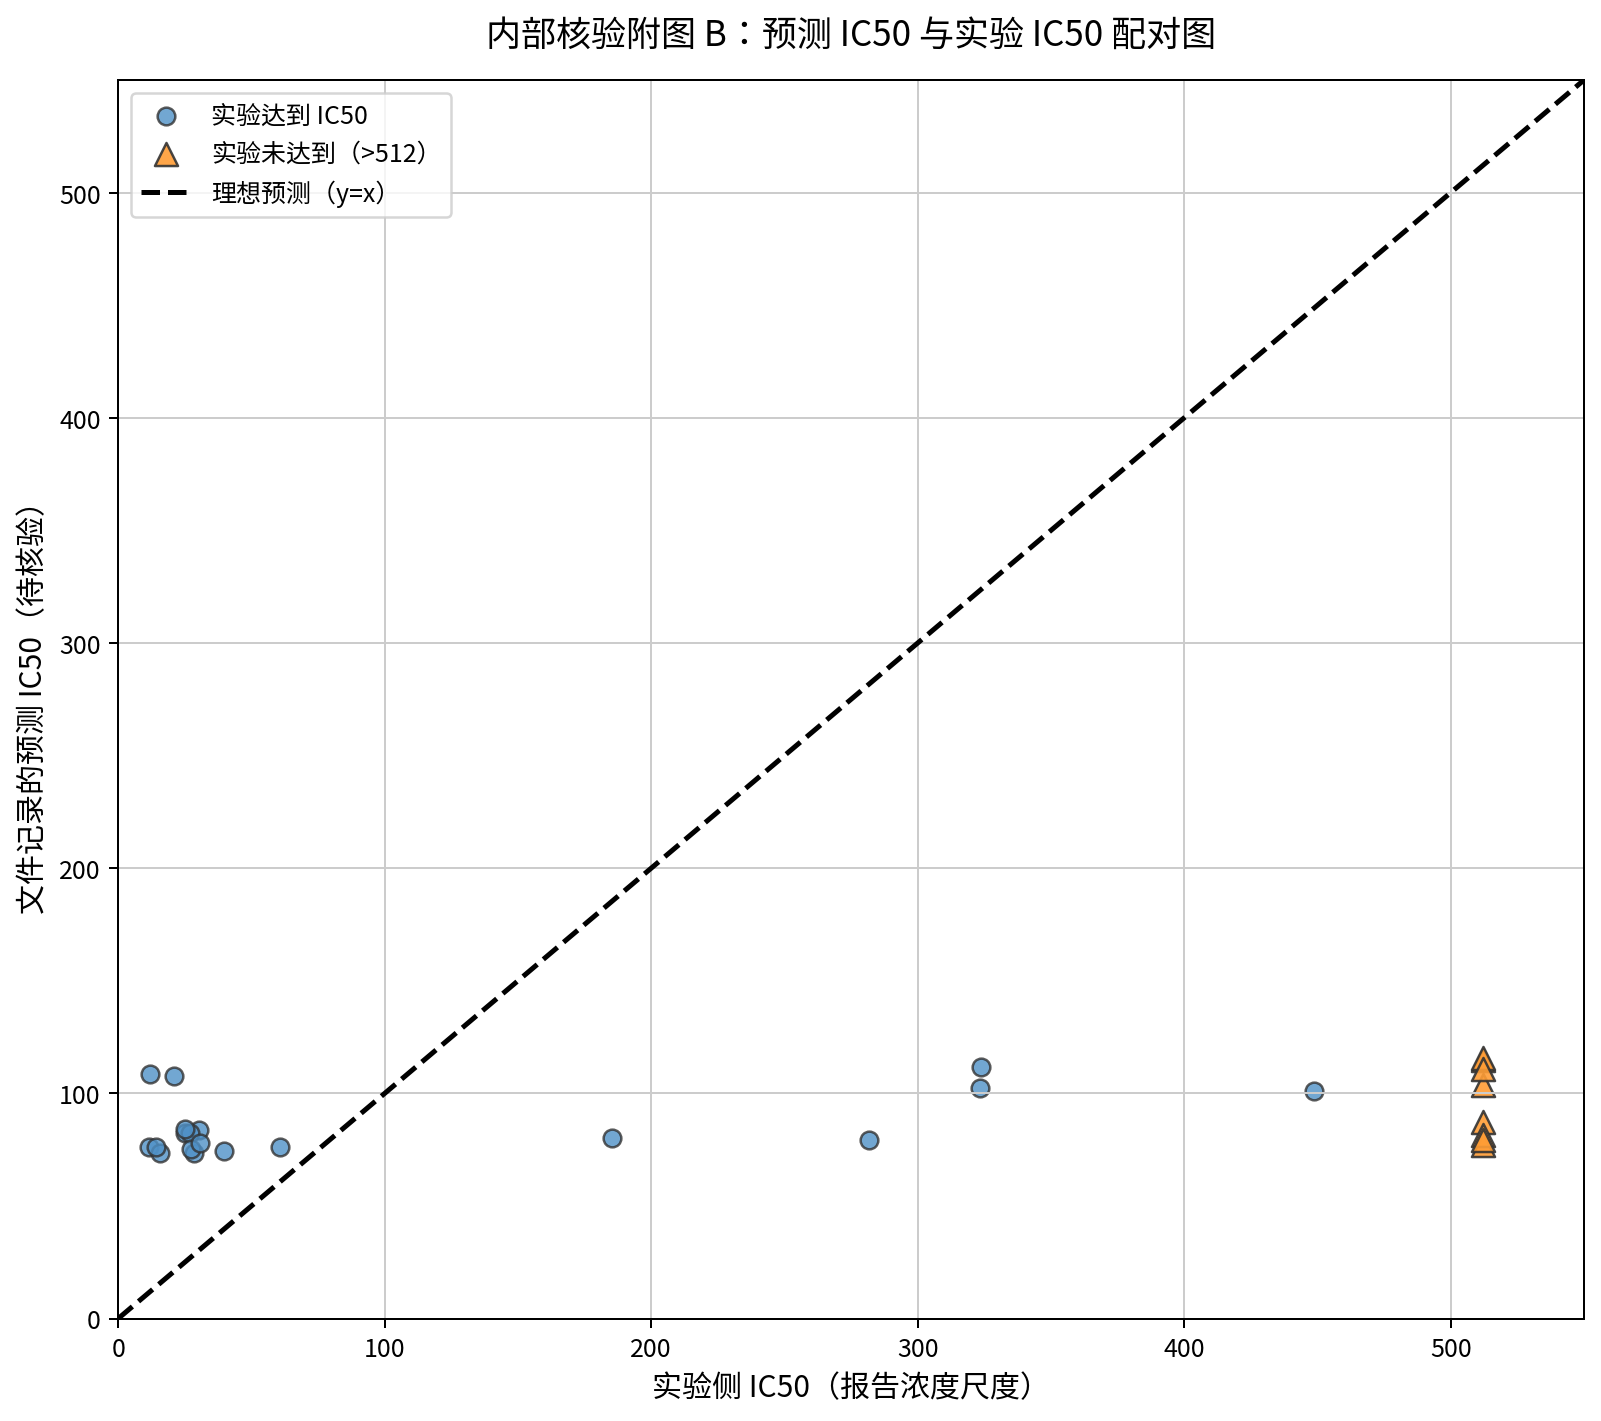
\includegraphics[width=\linewidth,height=0.70\textheight,keepaspectratio]{figures/word-20261021/ic50-pairing.png}
\caption*{内部核验附图 B. 预测 IC50 与实验 IC50 配对散点图。暂不纳入正式正文。预测曲线未跨越 50\% 存活率阈值，图中有限预测 IC50 及其配对误差目前缺少与曲线一致的可复现依据。}
\label{fig:huvec_internal_ic50}
\end{figure}

\subsection*{提交前仍需核验的事项}

% Word body block 149
核对实验浓度单位、元素硒计量基准及从报告浓度到模型输入浓度的换算方法。

% Word body block 150
补齐细胞来源、培养条件、检测方法、对照设置、归一化公式、技术重复和独立实验次数。

% Word body block 151
为 IAE 热图提供可复现的公式和计算脚本，并从预测—实测曲线重新计算。

% Word body block 152
移除或重新计算任务 26 中无法由预测曲线识别的 pred\_ic50、log\_error 及任何相关 R\textsuperscript{2}。

% Word body block 153
任务 30 的 SHAP 说明提到 shap\_code\_snippet.py，但当前附件中未提供该脚本正文。正式投稿前应随补充材料提供代码或稳定的代码存档入口。
